\section{Charakterystyka rynku}
	\par Należy tu scharakteryzować dwa rynki. Jednym z nich jest rynek polski, z którego to czerpane będą produkty oraz prowadzona będzie na nim sprzedaż dla klientów rodzimych. Drugim jest rynek kanadyjski, który będzie celem eksportu.

	\subsection{Rynek polski}
		\par Według badań przeprowadzonych przez Millward Brown,  rynek polski składa się 38.5 mln mieszkańców, z których 25.8 mln to internauci. 48\% z nich dokonało zakupów za pośrednictwem sklepów internetowych - daje to potencjalną grupę nabywców ok. 12 mln osób.  Jako, że statystycznie w Polsce mamy 14.1 mln. gospodarstw domowych, a 76\% z nich ma dostęp do internetu, to te 12 mln. potencjalnych nabywców mieszka w 10 mln. gospodarstw domowych. Średnia ilość internautów na gospodarstwo domowe 1.2. Jednocześnie rozwój branży mieszkaniowej sugeruje również wzrost na rodzimym rynku mebli. W pierwszym kwartale 2016 roku rozpoczęto budowę 133 tys. mieszkań, a branża odnotowała prawie 4\% wzrost.

		\begin{table}[H]
			\centering
			\begin{tabular}{|l|l|l|l|}
			\hline
																															& Miasto   & Wieś     & Razem    \\ \hline
			\begin{tabular}[c]{@{}l@{}}Liczba gospodarstw \\ domowych\end{tabular}               & 9400000  & 4700000  & 14100000 \\ \hline
			\begin{tabular}[c]{@{}l@{}}Liczba osób w gospodarstwach \\ domowych\end{tabular}     & 22842000 & 15322000 & 38164000 \\ \hline
			\begin{tabular}[c]{@{}l@{}}Średnia liczba osób\\ na gospodarstwo domowe\end{tabular} & 2.43     & 3.26     & 2.71     \\ \hline
			\end{tabular}
			\caption{Tabela dane dotyczące zamieszkania w Polsce}
			\label{avg_home_pl}
		\end{table}
	
		\par Rynek e-commerce w Polsce z roku na rok notuje coraz lepsze wyniki. Według badań przeprowadzonych przez Gemius, prawie połowa Polaków robi zakupy przez internet. W ich opinii zakupy on-line są wygodniejsze, tańsze, dostępne całą dobę i dają możliwość większego wyboru produktów. Wedle informacji zawartych w sprawozdaniu "Handel internetowy w Polsce 2015, analiza prognoza rozwoju rynku e-commerce  na lata 2015-2020", e-handel notuje stabilną dynamikę wzrostu, niezależnie od sytuacji na całym rynku detalicznym.
		
	
		\begin{figure}[H]
			\centering
			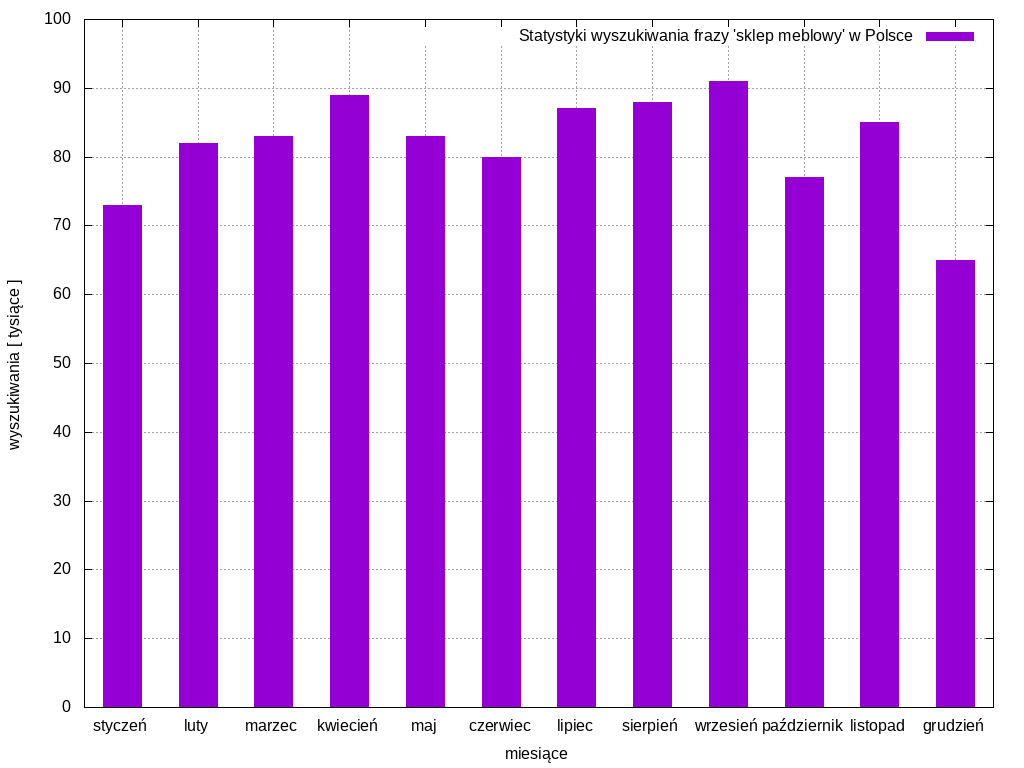
\includegraphics[scale=0.5]{stat_wysz_polska}
			\caption{Statystyki wyszukiwania frazy 'sklep meblowy' w Polsce}
			\label{search_pl}
		\end{figure}
	 
		\par Każdego miesiąca wedle statystyk "Google" w Polsce notowanych jest około 78 tyś. wyszukiwań frazy "sklep meblowy". Ludzie Ci to potencjalni klienci. Daje to sumarycznie prawie 1 mln. wyszukiwań rocznie. Na samym tylko "allegro.pl" korzystając z danych z ich magazynu, sprzedawanych jest dziennie ok. 2,5 tys. mebli dziennie. Biorąc pod uwagę, że według danych GUS mali producenci mebli (tzn. nie zatrudniający więcej jak 9 osób), posiadają  około 9\% całego polskiego rynku sprzedaży wewnętrznej. Daje to pule 90 tyś. klientów dla małych producentów mebli. Biorąc pod uwagę ilość małych producentów, według danych z 2010 roku około 13 tys. podmiotów daje około 6 klientów na podmiot. Zakładając średnią dla handlu internetowego w Polsce konwersję na 15\%,  aby uzyskać taką liczbę klientów należy ściągnąć na nią średnio 400 osób rocznie. Czyli 1.1 osoby dziennie, z czego 20\% stanowią meble do sypialni, 5\% stanowią meble kuchenne, a 75\% do salonów i jadalni.
		Bardziej szczegółowe dane prezentuje wykres.
	
	\subsection{Rynek kanadyjski}
		\par Rynek kanadyjski składa się z 31 mln. mieszkańców, z których 90\% tj. 27.9 mln. ludzi to internauci. Z handlu internetowego korzysta 51\% użytkowników, jest to ok. 14.3 mln. potencjalnych nabywców, z czego 34\% poszukuje w internecie mebli. Kanada liczy sobie 12.5 mln. gospodarstw domowych a średnia ilość ludzi w gospodarstwie wynosi 2.5.  Wynika z tego, że rynek stanowi 4.9 mln. użytkowników mieszkających w 1.96 mln. gospodarstw domowych. 

		\begin{table}[H]
		\centering
		\resizebox{\textwidth}{!}{%
		\begin{tabular}{|l|l|l|l|l|l|}
		\hline
																														& Domy jednorodzinne & \begin{tabular}[c]{@{}l@{}}Budynki apartamentowe \\ (powyżej 5 kondygnacji)\end{tabular} & Mieszkania ruchome & Inne    & Razem    \\ \hline
		\begin{tabular}[c]{@{}l@{}}Liczba gospodarstw\\ domowych\end{tabular}                 & 6871315            & 1114925                                                                                  & 163515             & 4285760 & 12435520 \\ \hline
		\begin{tabular}[c]{@{}l@{}}Liczba osób w \\ gospodarstwach domowych\end{tabular}      & 19310825           & 2030040                                                                                  & 365585             & 9365975 & 31072420 \\ \hline
		\begin{tabular}[c]{@{}l@{}}Średnia liczba osób \\ na gospodarstwo domowe\end{tabular} & 2.8                & 1.8                                                                                      & 2.2                & 2.2     & 2.5      \\ \hline
		\end{tabular}%
		}
		\caption{Dane statystyczne dotyczące zamieszkania w Kanadzie}
		\label{avg_home_ca}
		\end{table}

		\par Każdego miesiąca wedle statystyk "google" dla Kanady, fraza 'furniture store' wyszukiwana jest ok. 1 mln. przez unikalnych użytkowników. Są to użytkownicy poszukujący sklepów z meblami. Statystyka ta nie uwzględnia użytkowników korzystających z portali aukcyjnych. Na podstawie pozyskanych informacji, udało się ustalić, że 3.9 mln. użytkowników korzysta z portali aukcyjnych lub znanych stron przy zakupie mebli, a ok. 1 mln. klientów poszukuje nowych sklepów. Jednocześnie ze statystyk wynika, że udział polskich producentów w eksporcie produktów meblowych do Kanady wynosi 1.5\%. Daje to całkowitą pulę klientów 73.5 tyś. osób rocznie. Z braku danych statystycznych dla Kanady, przyjmijmy tu udział w rynku dla małych producentów podobny jak na rynku rodzimym tj. 9\%. Daje to 6.6 tyś. klientów rocznie. Rozkładając to na małych polskich producentów mebli, których jest 13.5 tyś. zakładając, (również z braku danych), że 25\% małych producentów eksportuje meble do Kanady daje to 1.95 klienta na podmiot rocznie. Aby osiągnąć nawet tak znikomą sprzedaż przy współczynniku konwersji 15\%, należy przyciągnąć do sklepu internetowego 13 unikalnych kanadyjskich użytkowników rocznie.
		
		\begin{figure}[H]
			\centering
			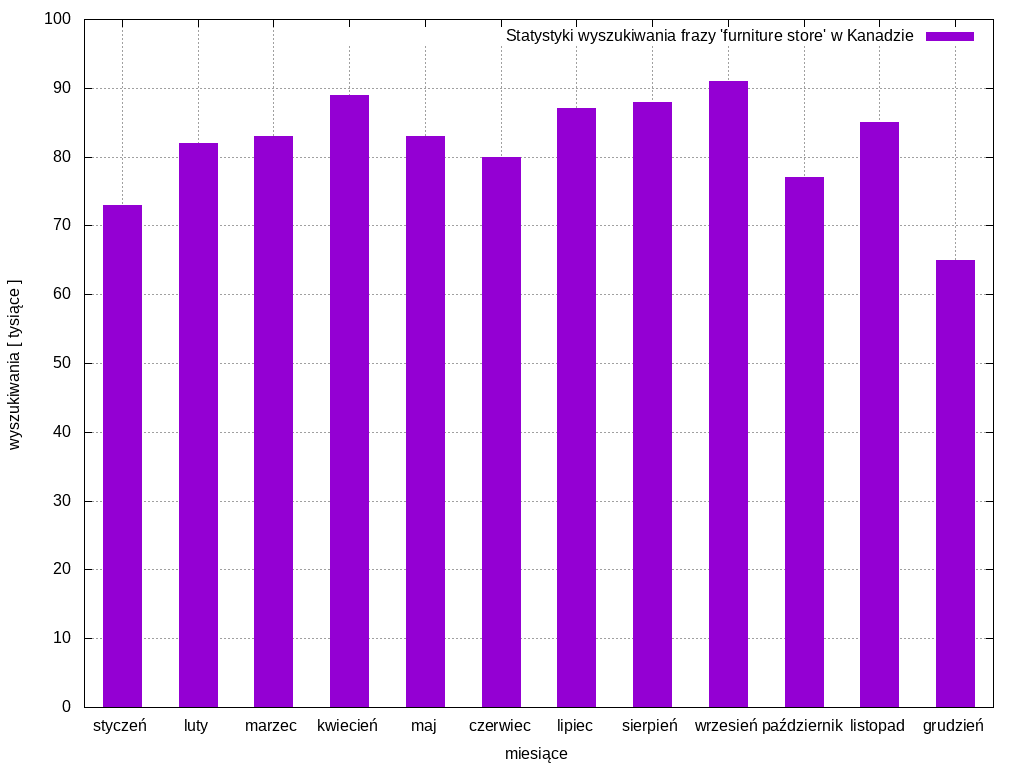
\includegraphics[scale=0.5]{stat_wysz_kanada}
			\caption{Statystyki wyszukiwania frazy 'furniture store' w Kanadzie}
		\end{figure}
	
	
	\section{Charakterystyka klientów}
		\subsection{Klienci indywidualani}
			\par Nabywcami w moim sklepie internetowym, będą oczywiście użytkownicy internetu. Należy ich podzielić na dwie kategorie: klientów polskich i klientów kanadyjskich.
			Według badań przeprowadzonych przez Millward Brown , w Polsce z internetu korzysta 76 procent obywateli, z czego 48 procent deklaruje, że chociaż raz w życiu dokonało zakupu za pośrednictwem internetu. W 2016 roku największą ilość nabywców na rynku e-commerce stanowiły osoby młode w wieku 25-35 lat, z wykształceniem średnim lub wyższym . To właśnie do nich będę przede wszystkim kierować swoją ofertę. Są to najczęściej osoby zabiegane ,które na co dzień  nie mają czasu na odwiedzanie sklepów stacjonarnych. Nabywców, którzy cenią sobie wysoką jakość produktu, jego oryginalność i niepowtarzalność.
			
			\par Osoby robiące zakupy online w powodach korzystania z tego rodzaju rozwiązania podają wygodę, oszczędność czasu i pieniędzy oraz większy wybór dostępnych produktów. Jako motywacje - 84\% podało dostępność całą dobę, 79\% brak konieczności jechania do sklepu, 75\% ceny atrakcyjniejsze niż w sklepach stacjonarnych. Dużym atutem była również dogodna forma dostawy i zwrotów.
			
			\par Eksport polskich mebli do Kanady działa coraz prężniej. Z najnowszych badań wynika, że na 35 milionów mieszkańców Kanady, aż 90\% jest czynnymi użytkownikami internetu. Kanadyjczycy bardzo chętnie kupują nasze rodzime meble drewniane, ze szczególnym wyróżnieniem mebli sypialnianych  oraz foteli, krzeseł i mebli tapicerowanych. Według moich spostrzeżeń jakie nabyłam podczas badania tamtejszego rynku, Kanadyjczycy gustują w pikowanych, skórzanych sofach, drewnianych , zdobionych łóżkach, dużych ,rodzinnych stołach. Mają duże zamiłowanie do folklorystycznych wzorów, których nie wyprodukują im duże zakłady stolarskie. Przede wszystkim takie produkty będę kierować za ocean.
					
		
	\section{Oczekiwania i potrzeby klientów}
		\par Z doświadczenia życiowego wynika, że klienci oczekują zakupu jak najlepszego produktu w jak najkorzystniejszej cenie. Głównym kryterium jest tu jednak jakość materiałów. Tkaniny obiciowe muszą być dobrej jakości, elementy drewniane muszą być dobrze, równomiernie wybarwione, a półki nie wypaczać się z czasem. Ważne jest również nie używanie plastikowych uchwytów do sprężyn w meblach tapicerowanych wykorzystywanych przez producentów na potęgę ze względu na niskie koszty. Niestety degradują się one w bardzo krótkim czasie co powoduje tzw. wychodzenie sprężyn i zapadnięcie mebla. Niezbędna jest więc kontrola jakości i inspekcja wizualna wysyłanego towaru. Jak udało się ustalić klienci są w stanie zapłacić więcej za dobrze wykonany produkt. Żyjemy w czasach gdzie rynki są przepełnione produktami z masowej produkcji, które nie zadowalają części klientów. Społeczeństwo polskie jak i zagraniczne corocznie się wzbogaca, dając nam tym samym wielkie pole do działania. Również sklepom internetowym. Przy tym bardzo ważny jest czas realizacji zlecenia, który musi zostać zminimalizowany. Kolejnym bardzo istotnym czynnikiem jest wspomniana już wcześniej możliwość personalizacji produktu. Klient musi mieć możliwość wyboru tkanin, wybarwień, rodzajów drewna lub wymiarów mebla. Sklep internetowy musi wychodzić naprzeciw oczekiwaniom klienta i umożliwiać personalizację mebli poczynając od materiałów a kończąc na detalach takich jak: nóżki, okucia czy chociażby guziki.
		
		
	\section{Analiza rynku}
		\par Na potrzeby polityki cenowej przeprowadzona została wstępna analiza rynku obejmująca badanie statystyczne najpopularniejszych portali aukcyjnych w Polsce i Kanadzie. Przebadane portale to ebay.ca i allegro.pl. Metodyką przeprowadzonej analizy było zestawienie pięciu par podobnych między sobą artykułów, a następnie wyliczenie na tej podstawie średniej arytmetycznej. Na podstawie przeprowadzonej analizy udało się ustalić następujące ceny średnie artykułów z danych grup:
		
		\begin{table}[H]
		\centering
		\begin{tabular}{|l|l|l|}
		\hline
					& Polska [zł] & Kanada [zł]\\ \hline
		Komody 	& 384  & 2613 \\ \hline
		Fotele 	& 1058 & 2943 \\ \hline
		Sofy   	& 3729 & 9611 \\ \hline
		Stoły  	& 1185 & 3366 \\ \hline
		Łóżka  	& 1355 & 6145 \\ \hline
		\end{tabular}
		\caption{Średnia cena grup produktów w Polsce i Kanadzie}
		\label{avg_grp_price_ca_pl}
		\end{table}

		Ponadto dzięki powziętej analizie udało się wyliczyć średnią cenę towarów Polsce jak i w Kanadzie. Średnia cena w Polsce wynosi 1831 zł, a w Kanadzie 5516 zł. Co daje różnicę w cenie średniej w wysokości 3685 zł. Jest potencjalny zarobek w przypadku eksportu. Jednak dla określenia polityki cenowej istotne jest jeszcze określenie średniej ceny transportu towaru od producenta do klienta. Na tę potrzebę przeprowadzono analizę dokładnie tą samą metodologią. Jej wyniki prezentuję tabela poniżej.
		
		\begin{table}[H]
		\centering
		\begin{tabular}{|l|l|l|l|}
		\hline
					& Polska \textless-\textgreater Polska [zł] & Kanada \textless-\textgreater Kanada [zł] & Polska \textless-\textgreater Kanada [zł] \\ \hline
		Komody 	& 69                                 & 414                                & 960                                \\ \hline
		Fotele 	& 51                                 & 408                                & 960                                \\ \hline
		Sofy   	& 480                                & 1225                               & 1606                               \\ \hline
		Stoły  	& 94                                 & 1137                               & 960                                \\ \hline
		Łóżka  	& 321                               	& 1167                               & 1200                               \\ \hline
		\end{tabular}
		\caption{Średnia cena transportu wybranych grup produktów}
		\label{avg_grp_shp_price}
		\end{table}
		
		Dzięki tej analizie ustalono, że średnia cena wysyłki towaru w Polsce wynosi 203zł, cena wysyłki w Kanadzie wynosi 870zł, a przesyłki z Polski do Kanady 1137zł. Na tej podstawie można ustalić średnią kwotę wysyłki produktu z Polski do Kanady, na którą składać się będą wysyłka z Polski do Kanady oraz wysyłka na terenie Kanady. Nie wlicza się w nią natomiast cena transportu w Polsce, ponieważ wybrane firmy spedycyjne dysponują własną flotą na terenie Polski. Na tej podstawie średni koszt wysyłki oszacować można na 2007 zł.
		
		Na podstawie powyższych analiz można sformułować ogólny zarys cen obowiązujących na rynku, polskim średnia cena produktu 1831 zł, a średni koszt transportu 203zł. Natomiast dla rynku kanadyjskiego 5516 zł, średni koszt transportu to 870zł, oraz przedstawić poniższą tabelę zawierającą ceny średnie powiększone o średni koszt transportu.
		
		\begin{table}[H]
		\centering
		\begin{tabular}{|l|l|l|}
		\hline
					& Polska [zł]& Kanada [zł]\\ \hline
		Komody 	& 453  & 3027 \\ \hline
		Fotele 	& 1109 & 3351 \\ \hline
		Sofy   	& 4209 & 10836 \\ \hline
		Stoły  	& 1279 & 4503 \\ \hline
		Łóżka  	& 1676 & 7312 \\ \hline
		\end{tabular}
		\caption{Średnia cena produktu w Polsce i Kanadzie powiększona o średni koszt transportu}
		\label{avg_price_pl_ca}
		\end{table}

		Na podstawie powyższych można ustalić  następującą politykę cen dla Polski i dla Kanady. Korzystając z danych GUS o polskim rynku wewnętrznym można ustalić marżę na 20\%. Co do rynku kanadyjskiego do ustalenia marży konieczne będzie wykorzystanie informacji ustalonych podczas analizy rynkowej.
		
		\begin{figure}[H]
			\centering
			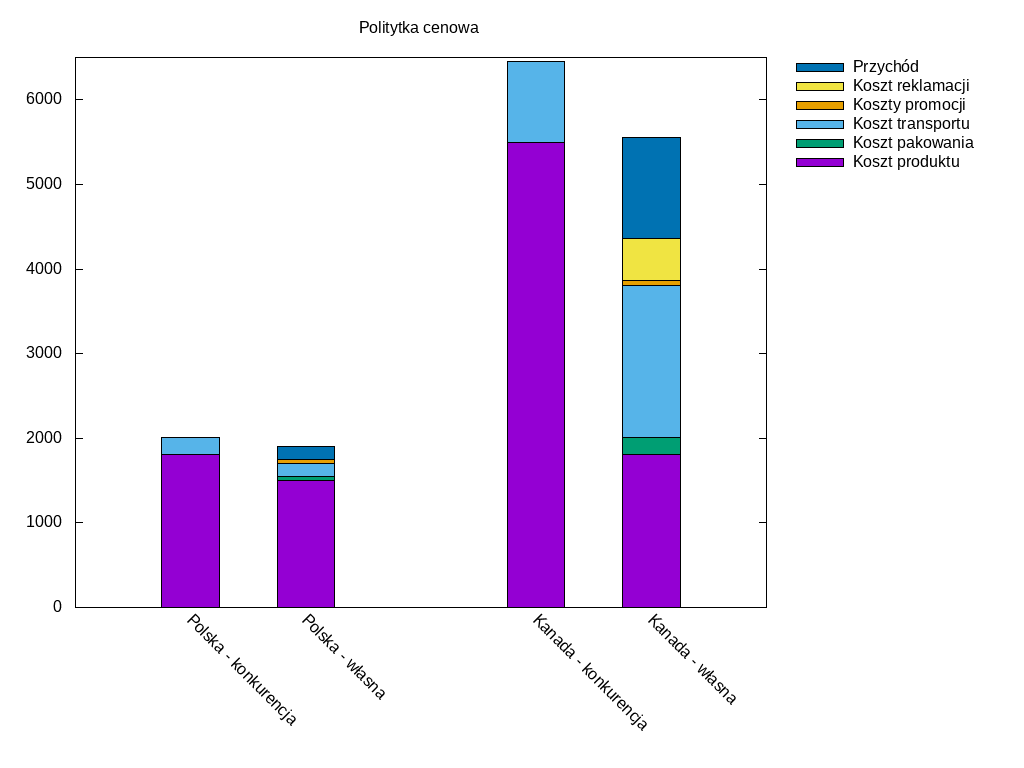
\includegraphics[scale=0.5]{polityka_cen}
			\caption{Polityka cenowa w Polsce i Kanadzie}
			\label{polityka_cen}
		\end{figure}

		W dziale charakterystyki rynku udało się ustalić średnią liczbę 6 klientów na producenta na rynku rodzimym, oraz średni przychód ze sprzedaży na 248 zł. Na rynku kanadyjskim natomiast średnią liczbę klientów na 1.95 klienta na podmiot. Biorąc pod uwagę dane z jednego producenta uzyskujemy przychód 1488 zł dla rynku polskiego. Dla rynku kanadyjskiego natomiast wyznaczono politykę cen na poziomie 80\% ceny konkurencji. Na podstawie ceny średniej w wysokości 5108 zł, udało się ustalić średni przychód w wysokości 910 zł. 

		\[ f(m) = (s_p \times p_p + s_k \times d_k ) \times m \]
		
		\begin{itemize}
			\item{\( s_p \)} średnia sprzedaż w Polsce na jednego producenta
			\item{\( d_p \)} średni dochód w Polsce ze sztuki sprzedanego towaru
			\item{\( s_k \)} średnia sprzedaż w Kanadzie na jednego producenta
			\item{\( d_k \)} średni dochód w Kanadzie ze sztuki sprzedanego towaru
			\item{m} liczba współpracujących producentów
		\end{itemize}
		
		Po podstawieniu parametrów i wyliczeniu otrzymujemy funkcję:
		
		\[	f(m) = 3262.5 \times m \]

		Wykres tej funkcji przedstawia przychód w zależności od ilości producentów przy założeniu osiągnięcia średniej sprzedaży.
		
		\begin{figure}
			\centering
			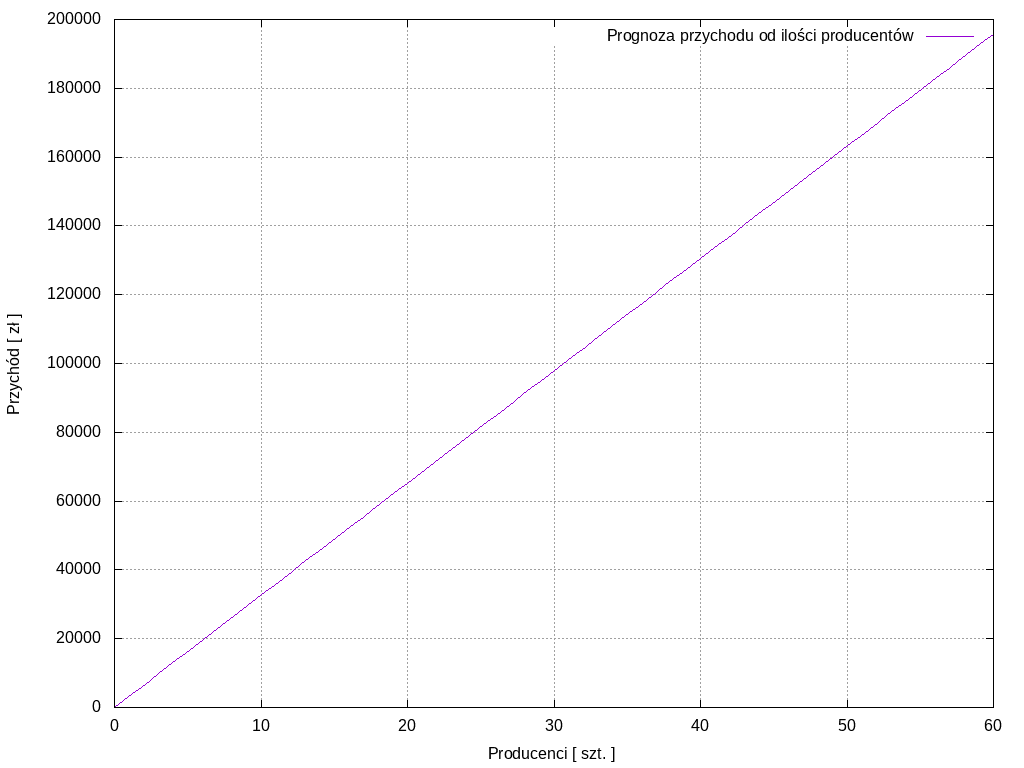
\includegraphics[scale=0.5]{income_prod}
			\caption{Wykres zależności przychodów od ilości producentów}
			\label{income_prod}
		\end{figure}

		Ważną informacją będzie też liczba odwiedzin potrzebna do osiągnięcia średniej sprzedaży. 
		
		\[ f(m) = \dfrac{ s_p + s_k }{w_k} \times m \] %konwersja
		
		\begin{figure}
			\centering
			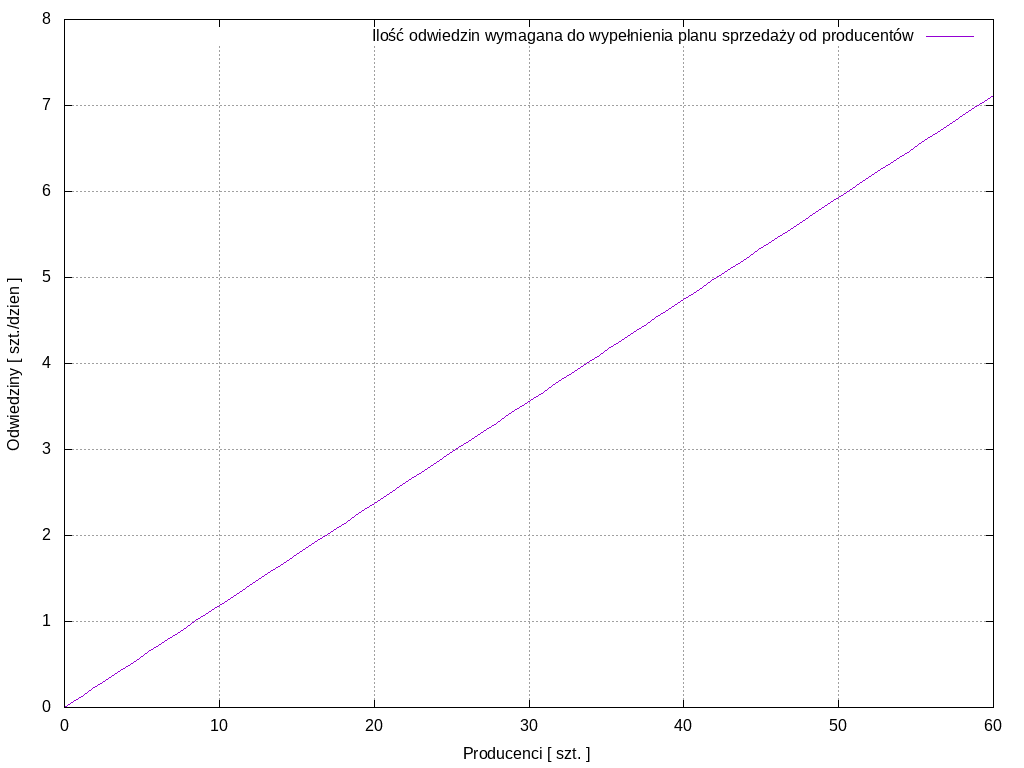
\includegraphics[scale=0.5]{visit_prod}
			\caption{Wykres zależności wymaganych do osiągnięcia średniej sprzedaży odwiedzin strony od producentów}
			\label{visit_prod}
		\end{figure}
		
		Wykresy \ref{income_prod} i \ref{visit_prod} powiązane są ze sobą w następujący sposób do osiągnięcia zakładanej sprzedaży przy danej ilości producentów potrzeba uzyskać przynajmniej taką ilość wejść na stronę od unikalnych potencjalnych klientów jak prezentuje drugi wykres.
		W poprzedniej części ustalono również, że 20\% sprzedaży stanowią meble do sypialni, 5\% stanowią meble kuchenne, a 75\% do salonów i jadalni.
		Ustalając liczbę producentów do pozyskania rocznie na 20 uzyskujemy przewidywany przychód w wysokości 65 tys. zł, który wedle podziału procentowego kategorii przyjmuje następującą postać 13 tys. zł z meble do sypialni, 3.25 tys. z mebli kuchennych, 48.75 tys. mebli do salonów i jadalni.  
		
		Dla kolejnych ustaleń należy jeszcze obliczyć średnią ilość sprzedanych mebli wyraża się ona wzorem:
		
		\[ f(m) = ( s_p + s_k ) \times m = 7.95 \times m \]
		
		\begin{figure}
			\centering
			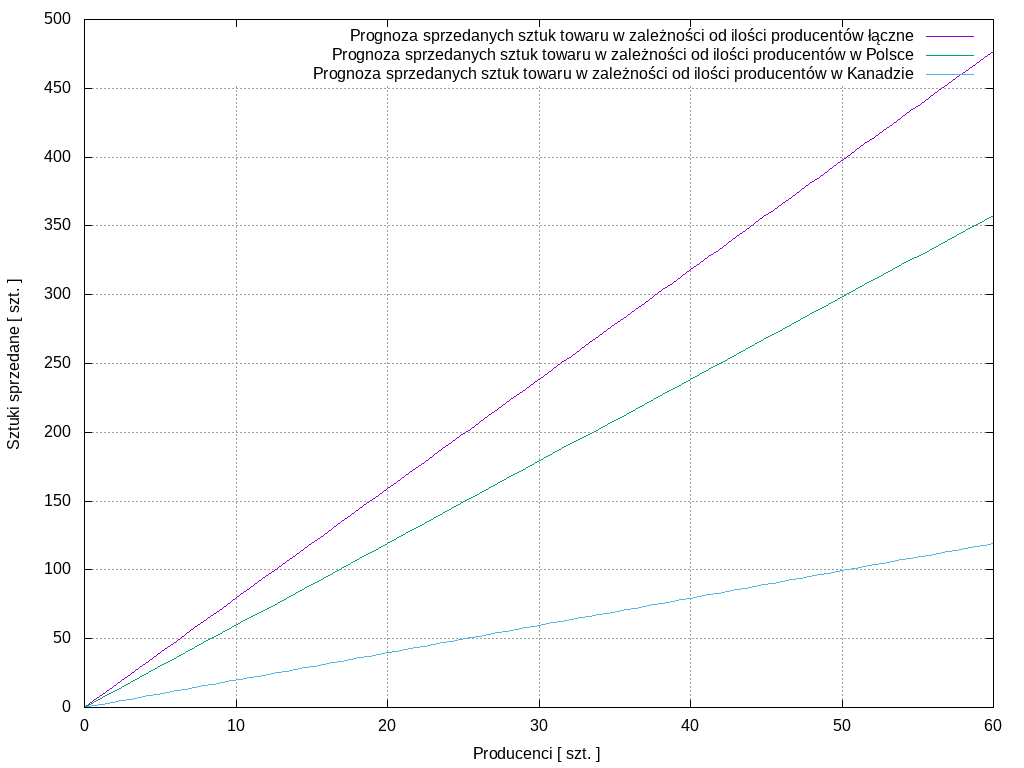
\includegraphics[scale=0.5]{sale_prod}
			\caption{Wykres wymaganej sprzedaży w sztukach od ilości producentów}
			\label{sale_prod}
		\end{figure}

		
	\section{Obecni konkurenci}
		\par W tym przypadku głównymi konkurentami nie są  duże sklepy meblowe, ale mniejsze oferujące niepowtarzalne meble hand-made. Jednym z nich jest sklep "bixbit.com", który posiada meble spersonalizowane o nowoczesnym wzornictwie. "Designconcept.pl" to kolejny sklep "www" oferujący  designerskie meble od różnych producentów. Nie można tu zapomnieć o jednym z największych konkurentów czyli "Meble.pl" działają na rynku od 2008 roku i przez ten czas zdobyli duże zaufanie klientów.
	
	
	\section{Sprzedaż i promocja}
		\par Sprzedaż będzie odbywała się poprzez sklep internetowy na dwóch domenach: sklep-meblowy.org oraz furniture-store.ca. Kluczowym było tu pozyskanie tych domen, ponieważ pozwoli to na zdobycie pozycji rynkowej małym nakładem finansowym. Domeny te to zlepki słów najczęściej wpisywanych według "Google" przez osoby szukające mebli w Polsce jak i w Kanadzie. Wyżej wymienione domeny są już moją własnością. Istotnym elementem sprzedaży i promocji jest wykorzystanie portali takich jak "ebay.ca", "amazon.com" oraz stosunkowo nowo powstały portal "ebid.net", który w samej Kanadzie zdobywa dużą popularność. Na rynku polskim należy skupić się również na portalach "allegro.pl" i "olx.pl"
	
		\par Pod kątem promocji sklepu i pozycjonowania, ważnym elementem jest wykorzystanie stron typu "gumtree.pl", "oglaszamy24.pl" ,"wykop.pl". Tej ostatniej odpowiednikiem o zasięgu globalnym jest "reddit.com".  Nieoceniona będzie również pomoc ze strony płatnych reklam w wyszukiwarce. Nie mówię tu jedynie o wyszukiwarce "google", należy skoncentrować też chociaż część wysiłków na wyszukiwarce wykorzystywanej domyślnie w produktach Microsoftu jaką jest "bing". Oczywiście nie można zapomnieć w tym miejscu o mediach społecznościowych jakimi są "facebook", "twitter" i "instagram", bez których nie da się już prowadzić biznesu. Mój sklep internetowy musi posiadać również  newsletter, który umożliwia rozsyłanie do zarejestrowanych klientów informacji o nowych produktach czy promocjach. W późniejszym etapie prowadzenia firmy, mam zamiar umieszczać reklamy w prasie branżowej np. "M jak mieszkanie", "Weranda" itp., na blogach wnętrzarskich, portalach poświęconych wystrojowi wnętrz. Istnieje też wiele wydarzeń np. targi meblowe, na których warto jest promować swoje produkty.
		
		
	\section{Dostawcy}
		\par Dostawcami w moim sklepie internetowym będą polscy wytwórcy mebli, którzy stawiają duży nacisk na wysoką jakość materiałów, precyzję wykonania i dbałość o najmniejszy szczegół. Zależy mi aby pozyskać małych producentów mebli, którzy swoje siedziby mają na terenie Dolnego Śląska. W trakcie badania rynku zauważyłam, że wiele małych przedsiębiorstw wykonuje niepowtarzalne przedmioty, które znalazłyby wielu nabywców, ale nie mają możliwości sprzedaży ich większej klienteli. 
		\par Dostawców mebli mam zamiar pozyskiwać poprzez przedstawienie im mojej oferty współpracy w sposób bezpośredni, za pośrednictwem portalu takiego jak "biznesoferty.pl", oraz poprzez przesyłanie im ulotki sklepu przygotowanej specjalnie na tą okoliczność.
		
	\section{Technologia i know-how}
		\par Technologią potrzebną dla poprowadzenia tego typu przedsiębiorstwa jest odpowiedni system komputerowy. W jego skład musi wchodzić system obsługi złożenia zamówienia, zarządzania procesem produkcji, oraz system kontroli wysyłki. System obsługi zamówienia musi przekazywać spójne dane dotyczące zamówienia złożonego przez klienta. Tu każdy produkt powinien dostać swój unikalny identyfikator na cały swój cykl życia. System zarządzania produkcją musi zawierać dane o czasie złożenia i zakończenia produkcji, oraz musi umożliwiać przepływ informacji między producentem a centralą firmy. Na samym końcu cyklu realizacji zamówienia system musi powiązać produkt po jego numerze seryjnym i adres klienta umożliwiając łatwe opatrzenie zapakowanego produktu danymi do wysyłki. Dzięki tak przygotowanemu systemowi centrala firmy będzie mieć kontrolę nad zamówieniem od momentu jego złożenia aż do dostarczenia dla klienta. System ten umożliwia też kontrolę jakości, nie tylko pod względem jakości jako takiej, ale również zgodności ze specyfikacją złożoną przez klienta.
		
		\par Dla prowadzenia tego typu działalności potrzebna jest podstawowa wiedza dotycząca prowadzenia firmy, kiedy wystawiać faktury, paragony, a kiedy ich oczekiwać. Przy przedsiębiorstwie eksportowym bardzo istotne jest odpowiednie prowadzenie dokumentacji zdarzeń gospodarczych.

		\par Przydatnym elementem systemów zarządzania jest narzędzie do planowania prac, obrazujące zadania i ich postęp za pomocą wykresu Gantt'a. Wykres pokazuje rozłożenie zadań do wykonania w czasie i osobami przypisanymi do zadań. Poniżej znajduje się przykładowy plan prac:

		
		
	
